% Entrega final (Fase 3) — Overleaf
% Subir a la raíz del proyecto Overleaf, junto con este main.tex:
%   logo_uexternado.png (opcional)
%   Carpeta entregables_para_informe/ con figuras (ver lista al inicio del cuerpo)
% Fuente base: segunda_entrega/Ml_segunda_entrega_final.pdf ≡ documentacion/segunda_entrega/main.tex

\documentclass[11pt]{article}
\usepackage[utf8]{inputenc}
\usepackage[T1]{fontenc}
\usepackage[margin=2.5cm]{geometry}
\usepackage{booktabs}
\usepackage{graphicx}
\usepackage{hyperref}
\usepackage{enumitem}
\usepackage{parskip}
\usepackage{float}
\usepackage{amsmath}
\usepackage{url}

\graphicspath{{entregables_para_informe/}}

\hypersetup{
    colorlinks=true, linkcolor=black, urlcolor=black, citecolor=black,
    pdftitle={Riesgo de incumplimiento crediticio - Entrega final},
    pdfauthor={Isabella Pensamiento, Juan Angel Triana}
}

\setlist[itemize]{leftmargin=1.4em, itemsep=1pt, topsep=2pt}
\setlist[enumerate]{leftmargin=1.6em, itemsep=1pt, topsep=2pt}

\renewcommand{\tablename}{Tabla}
\renewcommand{\figurename}{Figura}

\newcommand{\incluirlogo}{%
  \IfFileExists{logo_uexternado.png}{%
    
\includegraphics[width=6cm]{logo_uexternado.png}%
  }{%
    \vspace{2.5cm}{\small\textit{(Sube logo\_uexternado.png)}}%
  }%
}

\newcommand{\capturaapp}{%
  \IfFileExists{entregables_para_informe/captura_streamlit.png}{%
    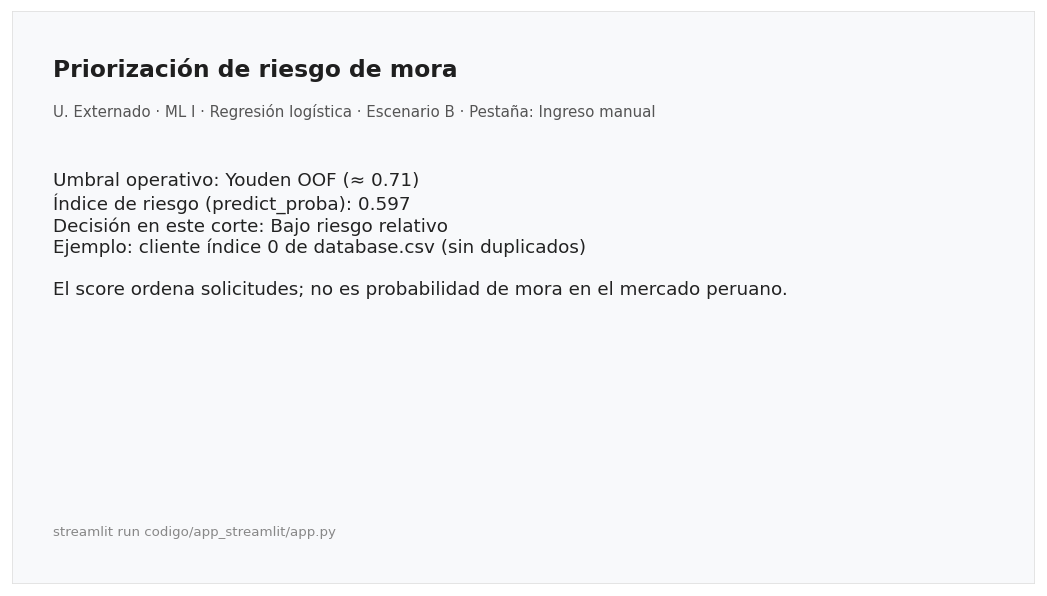
\includegraphics[width=0.88\textwidth]{captura_streamlit.png}%
  }{%
    \fbox{\parbox{0.85\textwidth}{\centering\vspace{2cm}\small Subir captura\_streamlit.png en entregables\_para\_informe/\vspace{2cm}}}%
  }%
}

\begin{document}

\begin{titlepage}
\centering
\incluirlogo
\vspace{0.7cm}

{\bfseries\large UNIVERSIDAD EXTERNADO DE COLOMBIA\par}
\vspace{2pt}
{\bfseries FACULTAD DE MATEMÁTICAS\par}
{PREGRADO EN CIENCIA DE DATOS\par}
\vspace{1.6cm}

\rule{\linewidth}{0.6pt}
\vspace{0.4cm}

{\Large\bfseries Riesgo de Incumplimiento Crediticio\par}
\vspace{0.3cm}
{\large Regresión Logística en el Contexto Latinoamericano\par}
\vspace{0.3cm}
{Entrega Final (Proyecto Integrador)\par}
\vspace{0.2cm}
{\normalsize Fase 3: consolidación, despliegue y comunicación\par}
\vspace{0.4cm}

\rule{\linewidth}{0.6pt}
\vspace{1.6cm}

{\large Isabella Pensamiento\par}
{\large Juan Angel Triana\par}
\vspace{0.8cm}

{\large Machine Learning I\par}
\vspace{0.3cm}
Profesora: Juliana De Mier
\vspace{2.5cm}

\vfill
{\bfseries Bogotá D.C. -- Colombia\par}
Noviembre de 2026
\end{titlepage}

\section{Decisión de negocio y alcance}

\textbf{Pregunta del comité.} ¿Podemos usar la información disponible de un solicitante para \textbf{priorizar clientes según riesgo relativo} sin rechazar innecesariamente demasiados buenos pagadores? La respuesta operativa depende del \textbf{umbral}, no solo del AUC.

\textbf{Pregunta técnica (heredada de la 2.ª entrega).} ¿Qué tan bien puede predecirse el riesgo de mora a partir de información financiera y socioeconómica disponible \emph{previamente}?

En esta entrega final \textbf{cerramos} la solución: un único modelo desplegable, reglas de uso honestas y umbrales orientados a costos de error. No agregamos QDA, Ridge ni Lasso para competir otra vez en el mismo conjunto de prueba.

\section{Limitaciones que condicionan cualquier lectura}

Las limitaciones van primero porque delimitan todo lo demás.

\begin{itemize}
\item \textbf{Temporalidad.} Sin fechas ni diccionario no demostramos que la etiqueta \texttt{mora} sea un evento futuro. Aprendemos a separar clientes ya marcados como morosos o pagadores al día con variables que \emph{suponemos} disponibles antes.
\item \textbf{Prevalencia.} En la muestra hay $\approx$71\% de mora. No es representativa del Perú (4\% a 11\% según la SBS). Los valores de \texttt{predict\_proba} sirven para \textbf{ordenar} riesgo en una población similar a esta base, no como probabilidad real de mora en el mercado.
\item \textbf{Identidad y duplicados.} No hay ID de cliente. Eliminamos duplicados exactos de forma conservadora, pero no sabemos si son la misma persona.
\item \textbf{\texttt{score}.} Lo mantenemos en el escenario principal y probamos el escenario C sin él. Si el score se actualizara después de atrasos, habría fuga residual no verificable sin metadatos.
\item \textbf{Conjunto de prueba.} En la 2.ª entrega usamos el 20\% de prueba para comparar modelos, escenarios y reportes con distintos cortes. Esa evaluación ya ocurrió. En la Fase 3 \textbf{no} reutilizamos test para elegir modelos ni umbrales nuevos. Solo repetimos cifras de cierre y aplicamos umbrales fijados en entrenamiento (OOF).
\end{itemize}

\section{Datos, fuga de información y escenario B}

Usamos \textit{BankDefaultAnalysis} (Kaggle, Calderón Baldeón, 2021): 8{,}399 registros, 13 predictores más \texttt{mora}. Tras quitar 2{,}325 filas duplicadas quedan 6{,}074 clientes. Partición 80/20 estratificada, semilla 42 (4{,}859 entrenamiento, 1{,}215 prueba).

Definición operativa: \texttt{mora = 1} es cliente marcado moroso en la base, \texttt{mora = 0} pagador al día. No afirmamos mora en un periodo exacto.

Excluimos \texttt{atraso} y \texttt{clasif\_sbs} del escenario principal porque describen comportamiento de pago y no podemos asegurar que se observen antes de la etiqueta. Escenario \textbf{B} (11 variables) es el modelo final. Escenarios A (13 variables) y C (sin \texttt{score}) se usaron en la 2.ª entrega como sensibilidad.

\section{Flujo de preprocesamiento y balanceo}

El preprocesamiento va en \texttt{Pipeline} (o \texttt{ImbPipeline} si hubiera balanceo): imputación mediana con indicador, estandarización, one-hot (\texttt{drop='first'}, \texttt{min\_frequency=50}), modelo. En validación cruzada cada fold ajusta transformaciones solo con su entrenamiento.

Probamos cinco estrategias de balanceo solo en entrenamiento (Tabla~\ref{tab:balanceo}). En \textbf{nuestro} experimento, ROC-AUC y PR-AUC en CV casi no cambian. Entrenamos el modelo final \textbf{sin balancear}. En general, remuestreo y pesos pueden alterar la frontera aprendida en otros contextos. Aquí el efecto visible al comparar opciones está sobre todo en recalls y tipos de error, no en discriminación global.

\begin{table}[H]
\centering
\caption{Balanceo en validación cruzada (regresión logística, escenario B), 2.ª entrega.}
\label{tab:balanceo}
\small
\begin{tabular}{@{}lcccc@{}}
\toprule
\textbf{Opción} & \textbf{AUC (CV)} & \textbf{PR-AUC (CV)} & \textbf{Rec. mora=1} & \textbf{Rec. mora=0} \\
\midrule
Sin balancear & 0,698 & 0,835 & 0,929 & 0,236 \\
Peso de clases & 0,699 & 0,836 & 0,682 & 0,612 \\
Submuestreo & 0,695 & 0,834 & 0,671 & 0,614 \\
Sobremuestreo & 0,698 & 0,836 & 0,679 & 0,608 \\
SMOTE & 0,695 & 0,834 & 0,665 & 0,616 \\
\bottomrule
\end{tabular}
\end{table}

\section{Modelo final y contraste con el artículo}

\subsection{Configuración definitiva}

\begin{table}[H]
\centering
\caption{Modelo final congelado (\texttt{contrato\_decisiones.md}).}
\label{tab:config}
\small
\begin{tabular}{@{}ll@{}}
\toprule
\textbf{Elemento} & \textbf{Valor} \\
\midrule
Algoritmo & Regresión logística (\texttt{C=1e6}, \texttt{max\_iter=5000}) \\
Variables & 11 (escenario B): perfil, \texttt{exp\_sf}, \texttt{linea\_sf}, \texttt{deuda\_sf}, \texttt{score}; sin \texttt{atraso} ni \texttt{clasif\_sbs} \\
Balanceo & Ninguno \\
Semilla & 42 \\
Salida operativa & Score de riesgo relativo (\texttt{predict\_proba[:,1]}) \\
Artefacto & \texttt{pipeline\_logistica\_B.joblib} \\
\bottomrule
\end{tabular}
\end{table}

\subsection{Por qué logística y no LDA, KNN o Naive Bayes}

La Tabla~\ref{tab:cv} (2.ª entrega) muestra AUC en CV: logística 0,698 $\pm$ 0,017, LDA 0,699, KNN 0,689 ($k=151$), Naive Bayes 0,657. Las diferencias entre los tres primeros son menores que la desviación entre folds. Naive Bayes queda peor, coherente con correlaciones entre variables financieras. Elegimos logística por \textbf{interpretabilidad} (logit y coeficientes) y alineación con el artículo de referencia (\textit{Credit/GoodBad}, regresión logística).

\subsection{Reproducción de objetivos del artículo}

\begin{itemize}
\item \textbf{Sí reproducimos en espíritu:} clasificación binaria de riesgo, métrica AUC, limpieza básica y logística como modelo interpretable en contexto latinoamericano (Perú).
\item \textbf{No reproducimos:} XGBoost, selección masiva de 541 variables, pipeline del paper a otra escala y país.
\item \textbf{Brecha de desempeño.} AUC en prueba $\approx$0,72 frente a objetivos más altos en el artículo. \textbf{Posibles razones no comprobadas:} muestra con 71\% de mora, escenario B sin variables de pago posteriores, ausencia de diccionario y calidad distinta a la del paper. Discriminación moderada (mejor que azar, lejos de separación perfecta). Un AUC de 0,72 \textbf{no} significa 72\% de aciertos.
\end{itemize}

\section{Validación cruzada (selección)}

\begin{table}[H]
\centering
\caption{AUC en validación cruzada (5 folds), escenario B. Fuente: 2.ª entrega / \texttt{tabla\_cv\_modelo\_final.csv}.}
\label{tab:cv}
\small
\begin{tabular}{@{}lcccc@{}}
\toprule
\textbf{Modelo} & \textbf{AUC (media)} & \textbf{Desv.} & \textbf{PR-AUC} & \textbf{Hiperparámetro} \\
\midrule
Regresión logística & 0,698 & 0,017 & 0,835 & --- \\
LDA & 0,699 & 0,017 & 0,835 & --- \\
KNN & 0,689 & 0,015 & 0,827 & $k = 151$ \\
Naive Bayes & 0,657 & 0,012 & 0,806 & --- \\
\bottomrule
\end{tabular}
\end{table}

\begin{table}[H]
\centering
\caption{AUC en CV (solo logística) por escenario de variables. Fase 3.}
\label{tab:cvabc}
\small
\begin{tabular}{@{}lc@{}}
\toprule
\textbf{Escenario} & \textbf{AUC CV} \\
\midrule
A. Completo (13) & 0,715 \\
B. Principal (11) & 0,698 \\
C. Conservador (sin \texttt{score}) & 0,692 \\
\bottomrule
\end{tabular}
\end{table}

\section{Evaluación en prueba (cierre congelado)}

En la 2.ª entrega consultamos el conjunto de prueba varias veces (modelos, escenarios y reportes con distintos cortes). Eso ya está documentado. En la Fase 3 \textbf{no} volvemos a usar test para \textbf{elegir} modelo ni umbral. Aquí repetimos las cifras de \textbf{cierre congelado} y verificamos que reentrenar el mismo pipeline reproduce AUC $\approx$0,722 (notebook \texttt{tercera\_entrega}).

\begin{table}[H]
\centering
\caption{Resultados en prueba (1{,}215 clientes), 2.ª entrega.}
\label{tab:test}
\footnotesize
\begin{tabular}{@{}lcccccc@{}}
\toprule
\textbf{Modelo} & \textbf{AUC} & \textbf{PR-AUC} & \textbf{Rec. mora=1} & \textbf{Prec. mora=1} & \textbf{Rec. mora=0} & \textbf{FN} \\
\midrule
Línea base & 0,500 & 0,710 & 1,000 & 0,710 & 0,000 & 0 \\
Regresión logística & 0,722 & 0,840 & 0,942 & 0,754 & 0,247 & 50 \\
LDA & 0,719 & 0,838 & 0,940 & 0,759 & 0,267 & 52 \\
KNN & 0,714 & 0,830 & 0,961 & 0,747 & 0,202 & 34 \\
Naive Bayes & 0,685 & 0,828 & 0,641 & 0,814 & 0,642 & 310 \\
Log.\ (Youden OOF) & 0,722 & 0,840 & 0,689 & 0,822 & 0,634 & 268 \\
\bottomrule
\end{tabular}
\end{table}

\noindent Las curvas de la Figura~\ref{fig:rocpr} resumen discriminación sin fijar umbral (cierre 2.ª entrega). Con prevalencia $\approx$71\% la PR-AUC alta refleja en parte la clase mayoritaria; el comité debe leer sensibilidad y falsos positivos al elegir corte.

\begin{figure}[H]
\centering
\begin{minipage}{0.48\textwidth}
\centering
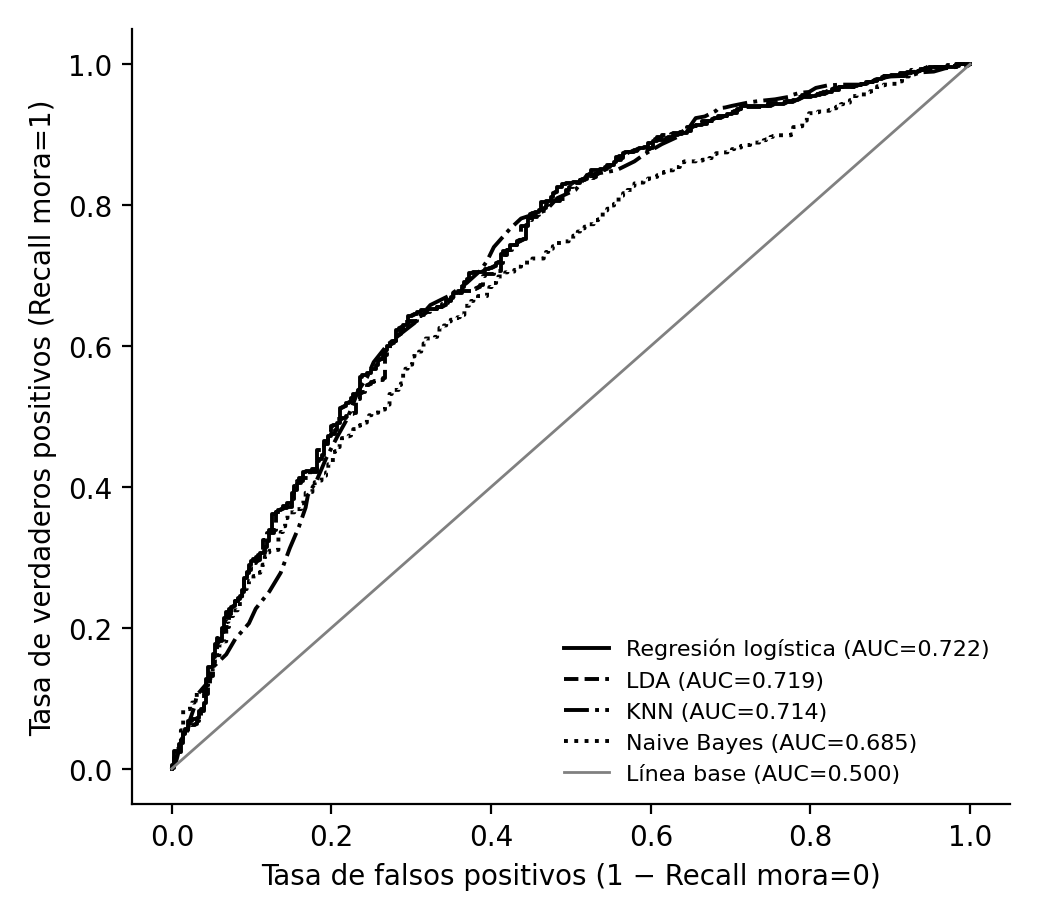
\includegraphics[width=\linewidth]{fig_roc.png}
\end{minipage}\hfill
\begin{minipage}{0.48\textwidth}
\centering
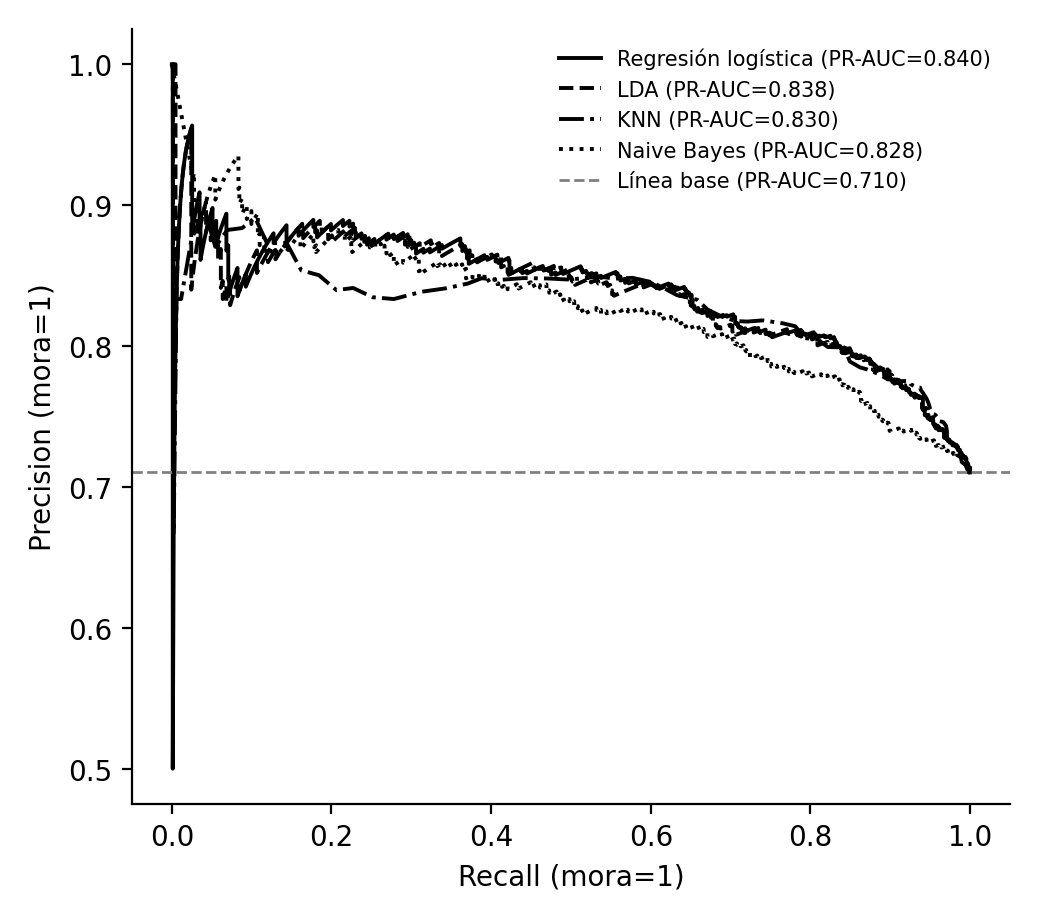
\includegraphics[width=\linewidth]{fig_pr.png}
\end{minipage}
\caption{ROC y precision--recall en prueba (regresión logística y comparadores, 2.ª entrega).}
\label{fig:rocpr}
\end{figure}

\section{Umbrales: Youden y escenarios de costo (OOF)}

La etiqueta binaria depende del umbral $t$ sobre el score del modelo. El índice de Youden $J = \mathrm{TPR} - \mathrm{FPR}$ se maximizó con probabilidades \emph{out-of-fold} en entrenamiento ($t \approx 0{,}71$).

Para la entrega final añadimos costos simbólicos $C = r \cdot FN + FP$ con $r =$ costo(FN)/costo(FP). Minimizamos $C$ en OOF (4{,}859 clientes de entrenamiento), sin mirar test. Incluimos $r \in \{1, 2, 5\}$ y la \textbf{línea base} que predice siempre mora (FN$=0$, FP$=$ buenos pagadores en OOF $=1{,}409$).

\begin{table}[H]
\centering
\caption{Umbrales y costo simbólico en OOF (entrenamiento, logística B). $C = r\cdot FN + FP$.}
\label{tab:costos_oof}
\footnotesize
\begin{tabular}{@{}lrrrrrrr@{}}
\toprule
\textbf{Criterio} & \textbf{$t$} & \textbf{FN} & \textbf{FP} & \textbf{$C$ $(r{=}1)$} & \textbf{$C$ $(r{=}2)$} & \textbf{$C$ $(r{=}5)$} & \textbf{Esp.} \\
\midrule
Línea base (siempre mora) & --- & 0 & 1409 & 1409 & 1409 & 1409 & 0,000 \\
Convención & 0,50 & 244 & 1076 & 1320 & 1564 & 2296 & 0,236 \\
Costo $r=1$ (mín. en OOF) & 0,57 & 381 & 921 & 1302 & 1683 & 2826 & 0,346 \\
Youden OOF & 0,71 & 1090 & 544 & 1634 & 2724 & 5994 & 0,614 \\
Costo $r=2$ (mín. en OOF) & 0,27 & 13 & 1366 & 1379 & 1392 & 1431 & 0,031 \\
Costo $r=5$ (mín. en OOF) & 0,14 & 0 & 1404 & 1404 & 1404 & 1404 & 0,004 \\
\bottomrule
\end{tabular}
\end{table}

La línea base fija $C = 1409$ para cualquier $r$ porque FN$=0$. Con $r=1$ el modelo reduce el costo total a 1302 frente a 1409: ahí el corte binario \textbf{sí} aporta frente a rechazar a todos. Con $r=2$ el costo mínimo (1392) queda apenas por debajo de la línea base; con $r=5$ el óptimo (1404) casi coincide con 1409 y la especificidad cae a 0,004 (casi todos marcados como mora). \textbf{Mensaje para el comité:} cuando el falso negativo se pesa mucho más que el falso positivo ($r=2$ o $r=5$), el mejor umbral en OOF empuja a una regla casi igual a la línea base. El modelo \textbf{solo aporta de forma clara} si los dos errores tienen costos del mismo orden ($r=1$) o si el comité usa el \textbf{score para ordenar} y umbrales intermedios (Youden, $r=1$), no solo el extremo $r=5$.

\begin{figure}[H]
\centering
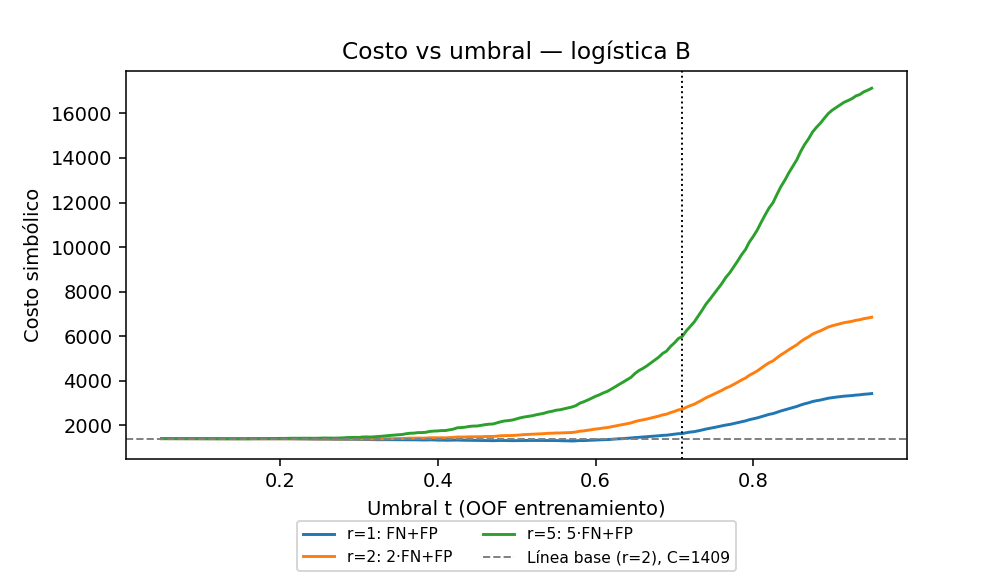
\includegraphics[width=0.92\textwidth]{fig_costo_vs_umbral.png}
\caption{Costo simbólico frente al umbral en OOF ($r=1$, $r=2$, $r=5$). Línea horizontal: línea base con $r=2$.}
\label{fig:costo}
\end{figure}

En prueba (solo lectura), con umbral 0,5 la logística deja 50 falsos negativos y reconoce 24,7\% de buenos pagadores. Con Youden OOF sube el reconocimiento de mora$=0$ al 63,4\%, con 268 FN.

\section{Robustez: escenario C y sensibilidad en prueba (2.ª entrega)}

\begin{table}[H]
\centering
\caption{AUC en prueba por escenario (comparación ya realizada en 2.ª entrega).}
\label{tab:sens}
\small
\begin{tabular}{@{}lccc@{}}
\toprule
\textbf{Modelo} & \textbf{A. Completo} & \textbf{B. Principal} & \textbf{C. sin score} \\
\midrule
Regresión logística & 0,734 & 0,722 & 0,709 \\
LDA & 0,730 & 0,719 & 0,707 \\
KNN & 0,721 & 0,714 & 0,702 \\
Naive Bayes & 0,692 & 0,685 & 0,677 \\
\bottomrule
\end{tabular}
\end{table}

Quitar \texttt{score} reduce poco el AUC. Mantenemos B pero documentamos la salvedad sobre el momento del \texttt{score}.

\section{Interpretación del modelo final}

Los coeficientes de la logística B (Figura~\ref{fig:coef}) son \textbf{asociaciones} en esta muestra, lineales en el \textbf{logit}. No son causas. Para un comité de riesgo, una lectura operativa es:

\begin{itemize}
\item \textbf{Score crediticio (\texttt{score}):} coeficiente negativo en logit $\Rightarrow$ un score más alto se asocia con \textbf{menor} índice de riesgo relativo del modelo. En lenguaje de comité: mejor historial resumido en \texttt{score} $\rightarrow$ prioridad de revisión más baja, \textbf{ceteris paribus}.
\item \textbf{Ahorro y estabilidad:} mayor \texttt{nivel\_ahorro}, más \texttt{exp\_sf} o más \texttt{dias\_lab} acompañan menor riesgo relativo; ayudan a ordenar cola de solicitudes, no sustituyen política de cupos.
\item \textbf{Carga de deuda:} mayor \texttt{deuda\_sf} $\rightarrow$ mayor riesgo relativo (más exposición en el sistema). Útil para alertar perfiles ya muy apalancados antes del desembolso.
\item \textbf{Perfil socioeconómico:} categorías de \texttt{vivienda}, \texttt{zona} y \texttt{nivel\_educ} se codifican respecto a referencias aprendidas en entrenamiento; un nivel educativo distinto al de referencia puede subir o bajar el logit en esta muestra.
\item \textbf{Odds ratio (lectura bancaria):} si el OR de una categoría es $>1$, en esta muestra ese grupo tuvo más mora que la referencia tras el ajuste lineal; si $<1$, menos. Son \textbf{asociaciones}, no causas ni montos en soles.
\item El modelo \textbf{ordena} la cartera para revisión manual; el comité define umbral, costos y excepciones.
\end{itemize}

\begin{figure}[H]
\centering
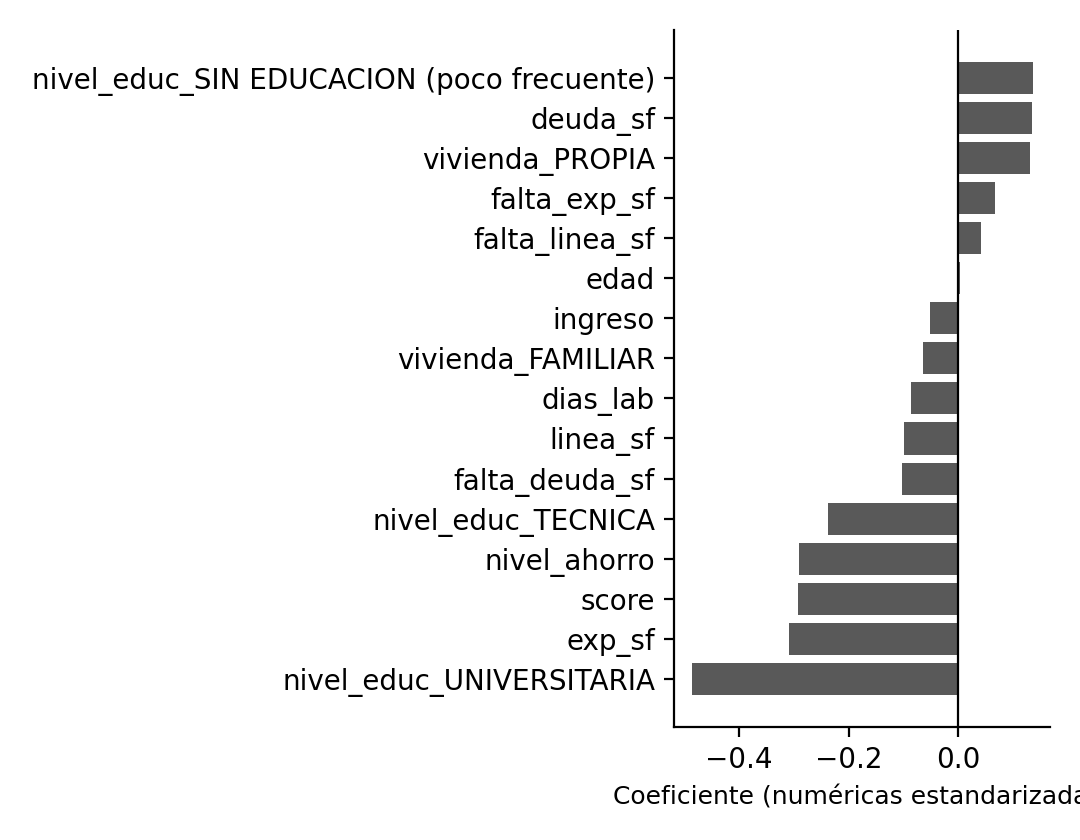
\includegraphics[width=0.88\textwidth]{fig_coeficientes.png}
\caption{Coeficientes de la regresión logística, escenario B.}
\label{fig:coef}
\end{figure}

\section{Despliegue básico (Streamlit)}

\textbf{Por qué Streamlit.} La guía de la Fase 3 (§8.3) exige un despliegue básico y funcional y sugiere, como ejemplo, una aplicación sencilla en Streamlit. Lo elegimos porque coincide con nuestro stack (Python, \texttt{scikit-learn}, \texttt{joblib}), permite en pocos archivos cargar el mismo pipeline entrenado, recoger las 11 entradas del escenario B, aplicar los umbrales del JSON y mostrar advertencias de limitación sin montar un backend aparte. Es adecuado para la \textbf{sustentación oral} (\texttt{streamlit run} en portátil) y para que el comité vea cómo cambia la decisión al mover el umbral. No pretendemos producción bancaria ni exposición pública de la API; es una demo reproducible alineada con la rúbrica de despliegue.

Implementamos la aplicación en \texttt{codigo/app\_streamlit/}. La app carga el mismo pipeline guardado (\texttt{pipeline\_logistica\_B.joblib}), solicita las \textbf{mismas 11 variables} del escenario B, aplica imputación, escalado y las \textbf{categorías que el modelo conoció en el entrenamiento} (\texttt{handle\_unknown=infrequent}), y lee los umbrales de \texttt{umbrales\_recomendados.json}. La salida es el índice de riesgo relativo y la clase según el corte (0,50, Youden, costo 1$\times$, 2$\times$ o 5$\times$). La interfaz muestra limitaciones en el panel lateral y, si el usuario elige costo 2$\times$ o 5$\times$, advierte que ese corte marca riesgo a casi todos (casi equivalente a rechazar a todos). Requiere \textbf{scikit-learn 1.9.1} e \textbf{imbalanced-learn 0.14.2} (ver README de la app).

\textbf{Ejecución local:}
\begin{verbatim}
pip install -r codigo/app_streamlit/requirements.txt
streamlit run codigo/app_streamlit/app.py
\end{verbatim}

\begin{figure}[H]
\centering
\capturaapp
\caption{Vista de la aplicación Streamlit (captura en \texttt{captura\_streamlit.png}).}
\label{fig:app}
\end{figure}

\section{Conclusiones y condiciones de uso}

\begin{itemize}
\item Con información previamente disponible y escenario B, la logística \textbf{ordena} mejor que la línea base (AUC $\approx$0,72, discriminación moderada).
\item El problema de negocio relevante es el \textbf{umbral}. Con $r=5$ la regla óptima en OOF casi coincide con la línea base. Con $r=1$ o Youden el modelo sí cambia el equilibrio de errores y sigue valiendo para \textbf{priorizar} por score.
\item \textbf{Recomendamos} usar el score del modelo para priorización interna en muestras similares si el comité acepta las limitaciones de temporalidad, prevalencia y \texttt{score}.
\item \textbf{No recomendamos} comunicar \texttt{predict\_proba} como probabilidad poblacional de mora en Perú ni tomar nuevas decisiones de modelo con el mismo test.
\end{itemize}

\textbf{Proyección (Machine Learning II).} Calibración de probabilidades, validación temporal con fechas, cost-sensitive learning con costos reales del banco y modelos más flexibles con control de sobreajuste.

\section*{Declaración de uso de inteligencia artificial}

Usamos el modelo de lenguaje \textbf{Claude (Sonnet 5)} de Anthropic, accedido vía Cursor, como apoyo para código, tablas y borradores del informe. El equipo revisó, ajustó y es responsable del contenido. El planteamiento, la base, las variables, el modelo final y la lectura de resultados son nuestros.

\section*{Referencias}

\begin{enumerate}[leftmargin=1.6em]
\item Attota, D. C., \& Yarmohammadtoosky, S. (2024). \textit{Optimizing Fintech Marketing: A Comparative Study of Logistic Regression and XGBoost}. Kennesaw State University. arXiv:2412.16333.
\item Calderón Baldeón, L. H. (2021). \textit{BankDefaultAnalysis: Morosidad del Sistema Financiero} [Conjunto de datos]. Kaggle. \url{https://doi.org/10.34740/KAGGLE/DSV/2528417}
\item Superintendencia de Banca, Seguros y AFP del Perú (SBS). (2021). \textit{Clasificación de riesgo crediticio y estadísticas de morosidad del sistema financiero peruano}. \url{https://www.sbs.gob.pe}
\item Anthropic. (2026). Claude (Sonnet 5) [Modelo de lenguaje de gran escala]. \url{https://claude.ai}
\end{enumerate}

\end{document}
